\titledquestion{Multiple Choices}

Each question has \textbf{one or more} correct answer(s). Select all the correct answer(s). For each question, you will get 0 points if you select one or more wrong answers, but you will get 1 point if you select a non-empty subset of the correct answers.

Write your answers in the following table.

%%%%%%%%%%%%%%%%%%%%%%%%%%%%%%%%%%%%%%%%%%%%%%%%%%%%%%%%%%%%%%%%%%%%%%%%%%%
% Note: The `LaTeX' way to answer a multiple-choices question is to replace `\choice'
% with `\choice', as what you did in the previous questions. However, there are 
% still many students who would like to handwrite their homework. To make TA's work 
% easier, you have to fill your selected choices in the table below, no matter whether 
% you use LaTeX or not.
%%%%%%%%%%%%%%%%%%%%%%%%%%%%%%%%%%%%%%%%%%%%%%%%%%%%%%%%%%%%%%%%%%%%%%%%%%%

\begin{table}[htbp]
	\centering
	\begin{tabular}{|p{1.7cm}|p{1.7cm}|p{1.7cm}|p{1.7cm}|p{1.7cm}|p{1.7cm}|p{1.7cm}|p{1.7cm}|p{1.7cm}|}
		\hline
		(a) & (b) & (c) & (d) & (e) & (f) \\
		\hline
		%%%%%%%%%%%%%%%%%%%%%%%%%%%%%%%%%%%%%%%%%%%%%%%%%%%%%%%%%%
		% YOUR ANSWER HERE.
		    &     &     &     &     &     \\
		%%%%%%%%%%%%%%%%%%%%%%%%%%%%%%%%%%%%%%%%%%%%%%%%%%%%%%%%%%
		\hline
	\end{tabular}
\end{table}

\begin{parts}
    \part[2] A planar graph is a graph which can be embedded in a plane i.e. you can find a way to put all vertices on the plane where the edges will not intersect with each other. Which of the statement(s) is/are correct?
    \begin{choices}
        \choice $\forall n\leq 5, K_n$ is planar. $K_n$ means the complete graph with $n$ vertices.
        \choice $K_6$ is not planar.
        \choice DAGs are planar.
        \choice A tree is planar.
        \choice Bipartite graphs are planar.
    \end{choices}

    \part[2] Given a graph $G=(V,E)$, $w(e)$ indicates the weight of edge $e$. Which of the statement(s) is/are correct?
    \begin{choices}
        \choice Both Kruskal's and Prim's algorithms can correctly find the MST even when $\exists e, w(e)<0$.
        \choice Suppose $G$ is connected and $|E| = \omega(|V|)$, $G$ has a unique MST if and only if $\forall e,e'\in E, w(e) = w(e') \Leftrightarrow e = e'$ i.e. weights of edges are distinct.
        \choice Suppose $G' = (V,E)$ is the same graph as $G$ with different weight function $v(e)$. If they share a same MST $T$, then $T$ is also the MST of $G$ with weights $u(e) = w(e) + v(e)$.
        \choice If $G$ contains multi-edges i.e. $G$ is not simple, then Kruskal's algorithm will fail but Prim's won't fail when finding MST.
    \end{choices}

	\part[2] Given a graph $G=(V,E)$, which of the following is(are) correct? 
	\begin{choices}
		\choice If $G$ is a complete graph with $4$ vertices, then the number of spanning trees of $G$ is $16$.
		\choice After Kruskal's algorithm, we choose $m$ edges, then the number of connected components of $G$ is $|V|-m$.
		\choice If $G$ is stored in adjacency matrix, then the total time complexity of Kruskal's algorithm can reach $\Theta(|V|^2+|E|\log|E|)$.
        \choice Suppose $G$ is connected and $|V| = |E|$, the maximum number of spanning trees of $G$ can reach $\Theta(|V|)$.
	\end{choices}
    
    \part[2] Let $G$ be a weighted undirected graph with positive weights where edge $e$ has weight $w_e\in \mathbb{R}^+$ for all $e \in E$. A new graph $G'$, which is a copy of $G$, and the weight of each edge $e$ in $G'$ is transformed using a function $f(w_e)$. Which of the following statements is/are true?

    \begin{choices} 
        \choice If $f(w_e) = w_e^2$, then any MST in $G$ is also an MST in $G'$.
        \choice If $f(w_e) = 2^{w_e}$, then any MST in $G$ is also an MST in $G'$.
        \choice If $f(w_e) = \frac1 {w_e}$, then any MST in $G$ is also an MST in $G'$.
        \choice If $f(w_e) = \log (w_e)$, then any MST in $G$ is also an MST in $G'$.
    \end{choices}

	\part[2] What is the number of spanning trees of following graph?

    \begin{center}
    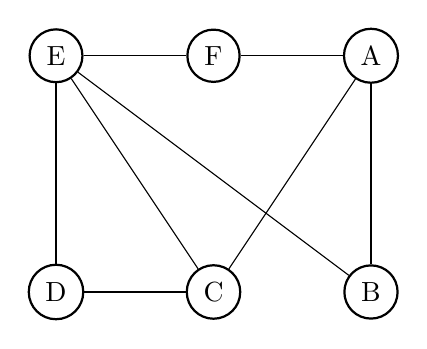
\begin{tikzpicture}
        \begin{scope}[every node/.style = {circle, thick, draw}]
            \node (A) at (2,0) {A};
            \node (B) at (2, -3) {B};
            \node (C) at (0, -3) {C};
            \node (D) at (-2, -3) {D};
            \node (E) at (-2, 0) {E};
            \node (F) at (0,0) {F};
        \end{scope}
        \begin{scope}
            \path[-] (E) edge (D);
            \path[-] (E) edge (C);
            \path[-] (E) edge (B);
            \path[-] (C) edge (D);
            \path[-] (B) edge (A);
            \path[-] (A) edge (C);
            \path[-] (A) edge (F);
            \path[-] (E) edge (F);
        \end{scope}
    \end{tikzpicture}
    \end{center}
	\begin{choices}
		\choice 32
		\choice 34
		\choice 36
		\choice 38
	\end{choices}

        \part[2] Which of the following statements are true for MST(Minimum Spanning Tree)?
        \begin{choices}
            \choice Suppose $G$ has multiple MSTs. For each minimum spanning tree $T$ of a graph $G$, there is a way to sort the edges of $G$ in Kruskal’s algorithm so that the algorithm returns $T$.
            \choice Prim's algorithm is a divide-and-conquer algorithm because it divides the graph into $S$ and $V-S$ then solve.
            \choice If we use binary heap to optimize Prim's algorithm when choosing the next edge, it will always have a better time complexity than the original algorithm on any graph.
            \choice If we add a new edge $e = (u,v)$ into a graph $G=(V,E)$ with unique MST to get a new graph $G' = (V,E\cup\{e\})$. There is at most $1$ edge difference between the MST of $G$ and $G'$.
        \end{choices}

\end{parts}
